\documentclass[a4paper]{article}
\usepackage[spanish,es-lcroman]{babel}
\usepackage[utf8]{inputenc}
\spanishdecimal{.}
\usepackage{bm}
\usepackage{amssymb}
\usepackage[margin=0.8in]{geometry}
\usepackage{parskip}
\usepackage{graphicx}
\usepackage{listings}
\usepackage{xcolor}
\usepackage{tikz}
\usepackage{multicol}
\usepackage{enumitem}
\usepackage{subcaption}
\definecolor{mygreen}{rgb}{0,0.6,0}
\definecolor{mypurple}{rgb}{0.7,0.3,0.7}
\lstset{
	language=Python,
	backgroundcolor=\color{white},
	frame=none,
	%
	basicstyle=\tt,
	commentstyle=\itshape\color{mygreen},
	keywordstyle=\color{magenta},
	identifierstyle=\color{cyan},
	stringstyle=\color{mypurple},
	showstringspaces=false,
	%
	numbers=none,
	%	numberstyle=\color{gray},
	firstnumber = 1,
	stepnumber=2,
	tabsize =2,
	%
	columns=flexible,
	breaklines=true
}
\lstset{
     literate=%
         {á}{{\'a}}1
         {í}{{\'i}}1
         {é}{{\'e}}1
         {ý}{{\'y}}1
         {ú}{{\'u}}1
         {ó}{{\'o}}1
         {ě}{{\v{e}}}1
         {š}{{\v{s}}}1
         {č}{{\v{c}}}1
         {ř}{{\v{r}}}1
         {ž}{{\v{z}}}1
         {ď}{{\v{d}}}1
         {ť}{{\v{t}}}1
         {ň}{{\v{n}}}1
         {ů}{{\r{u}}}1
         {Á}{{\'A}}1
         {Í}{{\'I}}1
         {É}{{\'E}}1
         {Ý}{{\'Y}}1
         {Ú}{{\'U}}1
         {Ó}{{\'O}}1
         {Ě}{{\v{E}}}1
         {Š}{{\v{S}}}1
         {Č}{{\v{C}}}1
         {Ř}{{\v{R}}}1
         {Ž}{{\v{Z}}}1
         {Ď}{{\v{D}}}1
         {Ť}{{\v{T}}}1
         {Ň}{{\v{N}}}1
         {Ů}{{\r{U}}}1      
         {s̄}{{\={s}}}1
         {ñ̄}{{\~{n}}}1
         {Ñ}{{\~{Ñ}}}1
}

\newenvironment{sidefig}[1]
{\noindent\begin{minipage}[c]{#1\textwidth}}
	{\vfill\end{minipage}}
\newcommand{\herefig}[1]{%
\end{minipage}
\hfill
\noindent\begin{minipage}[c]{#1\textwidth} 
	\centering\vfill
}

\author{Celia Rubio Madrigal}
\title{Práctica 3 - GCOMP}
\date{16 de marzo de 2022}

\begin{document}
	\maketitle
	
	\tableofcontents
	
	\vfill
	
	\begin{center}
			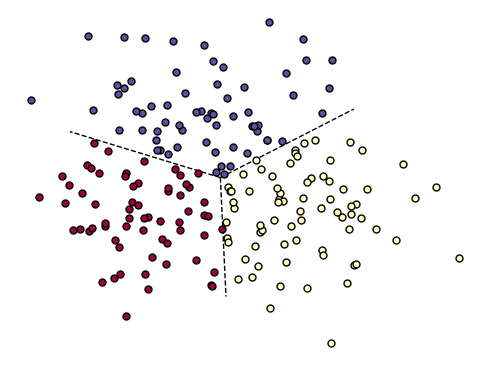
\includegraphics[width=0.66\linewidth]{portada}
	\end{center}
	
	
	\vfill
	\newpage
	
	\section{Introducción}
	En esta práctica aplicaremos algoritmos de clasificación no supervisada a un sistema dado. Suponemos que los elementos del sistema pueden agruparse en un número desconocido de clases en base a la distancia de sus estados frente a los del resto, y queremos responder las siguientes preguntas:
		¿Cuántas clases, o clústeres, forman los elementos?
		¿A qué clúster pertenece cada elemento?
		¿A qué clúster pertenecería un elemento nuevo?
	
	\section{Material usado y metodología}
	Partimos de un sistema de 1000 elementos con 2 estados cada uno, que generamos mediante la función \verb|make_blobs| a partir de 3 centros predefinidos: $(-0.5, 0.5)$, $(-1, -1)$ y $(1, -1)$.
	
	
	\subsection{Apartado \textit{i})}
	El primer algoritmo para agrupar los elementos del sistema es la clasificación por k-medias. Delimitará como clases las \textit{regiones de Voronoi} de unos puntos (los \textit{centroides}), que se deben determinar iterativamente.
	
	La región de Voronoi de un centroide $c$ será el conjunto de puntos del plano cuyo centroide más próximo sea $c$. Para poder definir la proximidad de los puntos usaremos la métrica euclídea sin ponderar, que es la p-norma con $p=2$ y pesos $w_i=1$: \(d_2(x,y) = \sqrt{\sum_{i=1}^2 |x_i-y_i|^2 }\). Así dividimos el espacio en regiones, y clasificamos los elementos del sistema según en qué región se encuentran sus estados.
	
	El algoritmo recibe como parámetros el número de centroides $k$ \textemdash igual al de clases\textemdash~ y los puntos del sistema. Mediante la clase \verb|KMeans| de \textit{sklearn}, y su método \verb+fit+, obtenemos en el atributo \verb+labels_+ la clasificación. Para averiguar cuál es el mejor $k$ debemos probar con valores en $[2,15]$ y calcular el coeficiente de Silhouette de cada clasificación. El coeficiente de Silhouette calcula si cada punto está bien clasificado en su clase con respecto a si estuviera en las otras clases. Nos quedaremos con el máximo, y dibujaremos los puntos ya clasificados junto a las fronteras de las regiones de Voronoi a las que pertenecen.
	
	
	\subsection{Apartado \textit{ii})}
	El segundo algoritmo de clasificación es DBSCAN, que basa sus agrupamientos en separar regiones de alta densidad de puntos mediante fronteras de baja densidad. Para ello, se toman bolas de un radio, o umbral de distancia, $\varepsilon$, y se van agregando puntos entre sí que son alcanzables mediante esas bolas. Se ha de tomar un límite para el que un elemento forma parte de la frontera de un clúster y no de su interior; será cuando no es alcanzable por otros $n_0=10$ puntos.
	
	El algoritmo recibe los puntos y el parámetro $\varepsilon$. Mediante la clase \verb|DBSCAN| de \textit{sklearn}, y su método \verb+fit+, obtenemos en \verb+labels_+ la clasificación. Para averiguar cuál es el mejor $\varepsilon$ debemos probar con valores en $(0.1,0.4)$ y calcular el coeficiente de Silhouette de cada clasificación, quedándonos de nuevo con el máximo. Las bolas pueden tomarse con distintas métricas. En nuestro caso serán la euclídea y la Manhattan (p-norma con $p=1$).
	
	\subsection{Apartado \textit{iii})}
	Con las celdas de Voronoi del apartado \textit{i}), podemos comprobar a cuáles pertenecerían otros elementos que no forman parte de nuestro sistema. Lo calculamos para $(0,0)$ y $(0,-1)$.
	
	\section{Resultados y conclusiones}
	
	\subsection{Apartado \textit{i})}
	Para los distintos valores de $k$, en la figura 1 se encuentran sus valores del coeficiente de Silhouette. El valor máximo es $k=3$ (\={s} $=0.588\pm 0.001$), que representamos en la figura 2. Los centroides resultantes son $(-0.54,0.50)$, $(-0.97,-1.02)$ y $(0.98,-0.98)$ $\pm 0.01$, que son muy cercanos a los tres puntos originales generadores del sistema.
	
	\begin{figure}[h!]\centering
\begin{minipage}{.4\textwidth}\label{fig:1}
	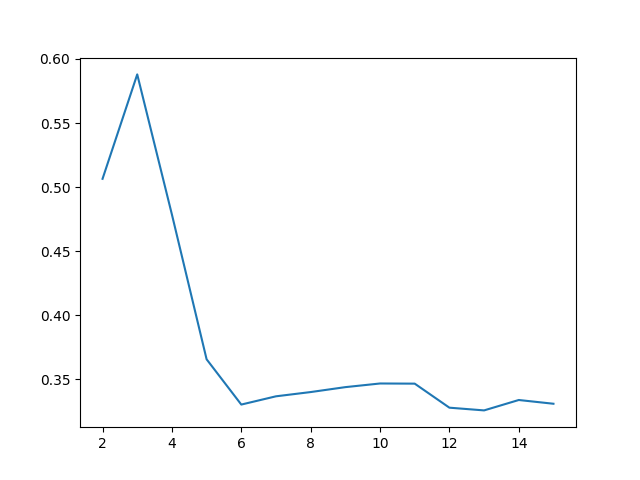
\includegraphics[width=\linewidth]{Figure_1}
	\captionof{figure}{Coefs. de Silhouette para KMeans con $k\in[2,15]$.}
	\end{minipage}\qquad
\begin{minipage}{.4\textwidth}\label{fig:2}
	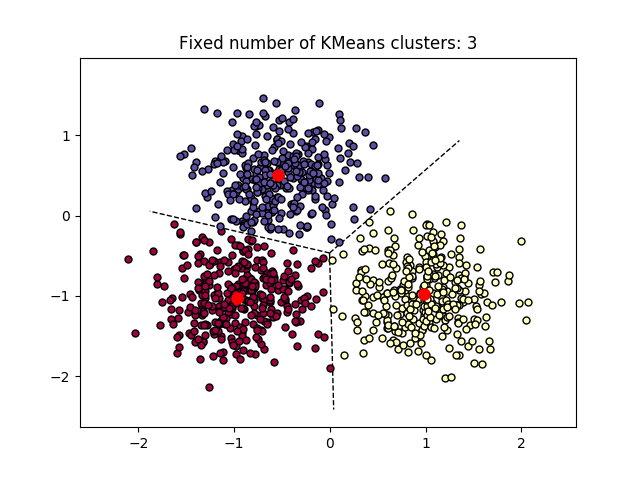
\includegraphics[width=\linewidth]{Figure_2}
	\captionof{figure}{Mejor clasificación del sistema mediante KMeans.}
	\end{minipage}
	\end{figure}

	\subsection{Apartado \textit{ii})}
	Para los distintos valores de $\varepsilon$, en la figura 3 se encuentran sus valores del coeficiente de Silhouette para la métrica euclídea (máximo en $\varepsilon=0.280\pm 0.001$, \={s} = 0.467$\pm 0.001$), y en la figura 5 para la Manhattan (máximo en $\varepsilon=0.320\pm 0.001$, \={s} = 0.440$\pm 0.001$). Las gráficas de sus clasificaciones están, respectivamente, en las figuras 4 y 6. 
	
	\begin{figure}[h!]\centering
\begin{minipage}{.4\textwidth}\label{fig:3}
	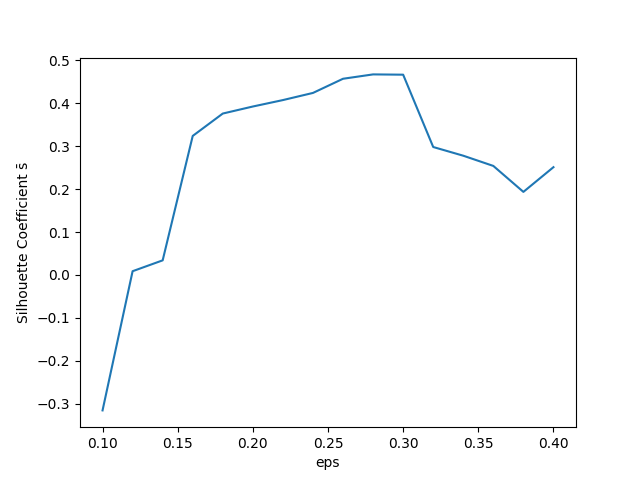
\includegraphics[width=\linewidth]{Figure_3}
	\captionof{figure}{Coefs. de Silhouette para DBSCAN euclídeo con $\varepsilon\in(0.1,0.4)$.}
	\end{minipage}\qquad
\begin{minipage}{.4\textwidth}\label{fig:4}
	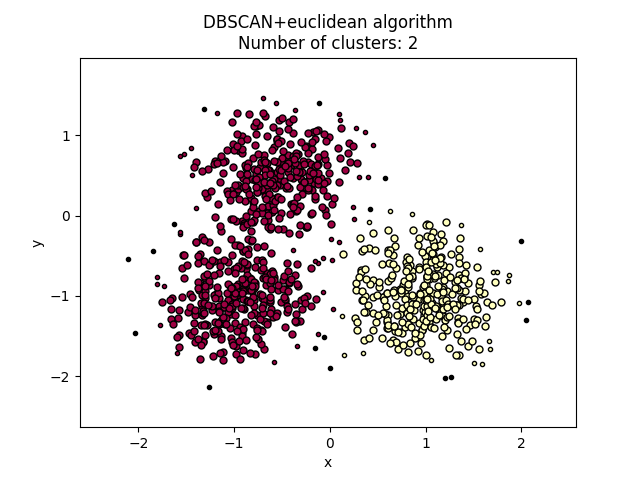
\includegraphics[width=\linewidth]{Figure_4}
	\captionof{figure}{Mejor clasificación mediante DBSCAN euclídeo.}
	\end{minipage}
	\end{figure}
	
	\begin{figure}[h!]\centering
\begin{minipage}{.4\textwidth}\label{fig:5}
	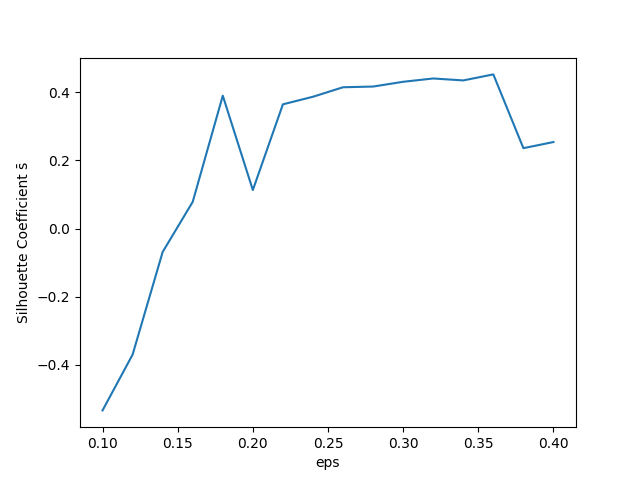
\includegraphics[width=\linewidth]{Figure_5}
	\captionof{figure}{Coefs. de Silhouette para DBSCAN Manhattan con $\varepsilon\in(0.1,0.4)$.}
	\end{minipage}\qquad
\begin{minipage}{.4\textwidth}\label{fig:6}
	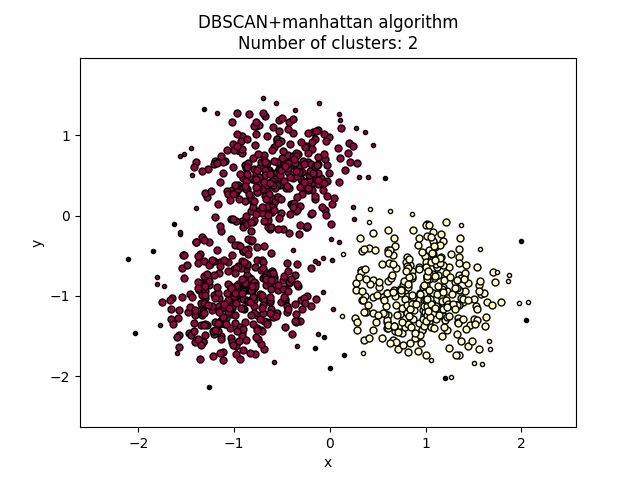
\includegraphics[width=\linewidth]{Figure_6}
	\captionof{figure}{Mejor clasificación mediante DBSCAN Manhattan.}
	\end{minipage}
	\end{figure}
	
	Hay 2 clases en vez de 3, ya que la frontera entre las dos a la izquierda es demasiado densa como para distinguirse mediante este algoritmo. También observamos que con este algoritmo algunos puntos son clasificados directamente como ruido en negro.
	
	\subsection{Apartado \textit{iii})}
	Volviendo a mirar la figura 1, un elemento con estado $(0,0)$ queda clasificado en el clúster azul. Sin embargo, $(0,-1)$ queda en la frontera de dos celdas de Voronoi. Por tanto, en algunas ejecuciones del comando \verb+kmeans.predict+ sale el clúster rojo y en otras el amarillo.
	
	\newpage
	\section{Código}\label{codigo}
	
	\lstinputlisting[language=Python]{p3_rubiomadrigalcelia.py}
	
\end{document}
